%% LyX 2.0.0rc3 created this file.  For more info, see http://www.lyx.org/.
%% Do not edit unless you really know what you are doing.
\documentclass[english]{beamer}
\usepackage{mathptmx}
\renewcommand{\familydefault}{\rmdefault}
\usepackage[T1]{fontenc}
\usepackage[latin9]{inputenc}
\usepackage{textcomp}
\usepackage{amsmath}
\usepackage{amssymb}
\usepackage{graphicx}

\makeatletter

%%%%%%%%%%%%%%%%%%%%%%%%%%%%%% LyX specific LaTeX commands.
%% Because html converters don't know tabularnewline
\providecommand{\tabularnewline}{\\}

%%%%%%%%%%%%%%%%%%%%%%%%%%%%%% Textclass specific LaTeX commands.
 % this default might be overridden by plain title style
 \newcommand\makebeamertitle{\frame{\maketitle}}%
 \AtBeginDocument{
   \let\origtableofcontents=\tableofcontents
   \def\tableofcontents{\@ifnextchar[{\origtableofcontents}{\gobbletableofcontents}}
   \def\gobbletableofcontents#1{\origtableofcontents}
 }

%%%%%%%%%%%%%%%%%%%%%%%%%%%%%% User specified LaTeX commands.
\usepackage{amsfonts}

\usetheme{Madrid}

%\usetheme{Warsaw}
% or ...

%\setbeamercovered{transparent}
% or whatever (possibly just delete it)

\newcounter{esr}
\newtheorem{esercizio}[esr]{Exercise}
\newcounter{osservcounter}
\newtheorem{osservazione}[osservcounter]{Remark}

\makeatother

\usepackage{babel}
\begin{document}

\title{Statistics Lecture}


\author{Claudio Ortelli~\inst{1}}


\institute{\inst{1} Finance Institute\\
Universit� della Svizzera italiana}


\date[ALARI 2011]{Advanced Learning and Research Institute, 2011}

\makebeamertitle
\section{Conditional distribution and expectation}

\begin{frame}{Conditional Distribution and Expectation}

Let $A$ and $B$ be two events and $P(B)\neq0$. The conditional
probability of the event $A$, given that event $B$ is realized,
is by definition 

\[
P(A\mid B)=\frac{P(A\cap B)}{P(B)}.
\]
Let $X$ be a random variable and define \textbf{$B$} to be the event
that $X=x$. The conditional probability $P(A\mid X=x)$ of the event
$A$ is then 
\[
P(A\mid X=x)=\frac{P(A\mbox{ and }X=x)}{P(X=x)}=\frac{P(A\cap[X=x])}{P(X=x)}=
\]
provided of course that $P(X=x)\neq0$.

\end{frame} 

\begin{frame}{Conditional Distribution and Expectation}
\begin{definition}%{}
\textbf{1) Conditional pmf}. Let $X$ and $Y$ be discrete random
variables with joint pmf $p(x,y)$. The conditional pmf of $Y$ given
$X$ is

\begin{eqnarray*}
p_{Y\mid X}(y\mid x) & = & P(Y=y\mid X=x)\\
 & = & \frac{P(Y=y,X=x)}{P(X=x)}=\frac{p(x,y)}{p_{x}(x)}
\end{eqnarray*}
if $p_{X}(x)\neq0$ and $0$ otherwise.

\textbf{2) The conditional distribution function} of a random Variable
$Y$ (not necessarily descrete) given a discrete random variable $X$
is

\[
F_{Y\mid X}(y\mid x)=P(Y\leq y\mid X=x)=\frac{P(Y\leq y\mbox{ and }X=x)}{P(X=x)}
\]
for all $y$ and all $x$ such that $P(X=x)\neq0$.
\end{definition}%{}
\end{frame} 

\begin{frame}{Conditional Distribution and Expectation}
\begin{example}%{}

\begin{itemize}
\item Server cluster with two servers labeled $A$ and $B$.
\item Incoming jobs are independently routed to $A$ and $B$ with probability
$p$ and $q=1-p$, respectively.
\item The number $X$ of arriving jobs per unit of time is Poisson distributed
with intensity $\lambda$. 
\item Determine the number of jobs, $Y$, received by server $A$, per unit
of time.
\end{itemize}
\[
P_{Y\mid X}(k,n)=\begin{cases}
P_{Y\mid X}(Y=k,X=n)=\left(\begin{array}{c}
n\\
k
\end{array}\right)p^{k}q^{n-k}, & 0\leq k\leq n.\\
0 & \mbox{otherwise.}
\end{cases}
\]

\end{example}%{}
\end{frame} 

\begin{frame}{Conditional Distribution and Expectation}
\begin{example}%{}
(Continued) Recall that $P(X=n)=e^{-\lambda}\lambda^{n}/n!$ so that
\begin{eqnarray*}
p_{Y}(k) & = & \sum_{n=k}^{\infty}p_{Y\mid X}(k\mid n)p_{X}(n)\\
 & = & \sum_{n=k}^{\infty}\left(\begin{array}{c}
n\\
k
\end{array}\right)p^{k}q^{n-k}\frac{e^{-\lambda}\lambda^{n}}{n!}\\
 & = & \lambda^{k}p^{k}e^{-\lambda}\sum_{n=k}^{\infty}\left(\begin{array}{c}
n\\
k
\end{array}\right)\frac{1}{n!}q^{n-k}\lambda^{n-k}\\
 & = & \frac{\left(\lambda p\right)^{k}}{k!}e^{-\lambda}\sum_{n=k}^{\infty}\frac{\left(q\lambda\right)^{n-k}}{(n-k)!}
\end{eqnarray*}
so that finally $p_{Y}(k)=\frac{\left(\lambda p\right)^{k}}{k!}e^{-\lambda}e^{q\lambda}=\frac{\left(\lambda p\right)^{k}}{k!}e^{-\lambda p}$,
i.e. $Y$ is Poisson distributed with intensity $\lambda p$.
\end{example}%{}
\end{frame}

\begin{frame}{Conditional Distribution and Expectation}

If $X$ is a continuous random variable then $P(X=x)=0$ for all $x\in\mathbb{R}$
so that the previous definition $\frac{P(Y=y,X=x)}{P(X=x)}$ of conditional
probability is not satisfactory.

However when $X$ and $Y$ are jointly continuous we can define the
conditional pdf of $Y$ given $X$:\medskip{}

\begin{definition}%{}
Let $X$ and $Y$ be continuous r.v. with joint pdf $f(x,y).$ The
conditional density $f_{Y\mid X}$ is 

\[
f_{Y\mid X}(y\mid x)=\begin{cases}
\frac{f(x,y)}{f_{X}(x)}, & \mbox{if }0<f_{X}(x)<\infty,\\
0 & \mbox{otherwise.}
\end{cases}
\]

\end{definition}%{}
\end{frame}

\begin{frame}{Conditional Distribution and Expectation}

From the definition of conditional density it follows that

\[
f(x,y)=f_{Y\mid X}(y\mid x)f_{X}(x)=f_{X\mid Y}(x\mid y)f_{Y}(y),
\]


and if $X$ and $Y$ are independent, then 
\[
f(x,y)=f_{X}(x)f_{Y}(y).
\]
Furthermore,
\[
f_{Y}(y)=\int_{-\infty}^{\infty}f(x,y)dx=\int_{-\infty}^{\infty}f_{Y\mid X}(y\mid x)f_{X}(x)dx
\]
which is the continuous analog of the thorem of total probability.

\end{frame}

\begin{frame}{Conditional Distribution and Expectation}
\begin{itemize}
\item The conditional pdf can be used to obtain the conditional probability:
\[
P(a\leq Y\leq b\mid X=x)=\int_{a}^{b}f_{Y\mid X}(y\mid x)dy,\qquad a\leq b.
\]

\item The conditional distribution function is defined analogously
\begin{eqnarray*}
F_{Y\mid X}(y\mid x) & = & P(Y\leq y\mid X=x)\\
 & = & \frac{\int_{-\infty}^{y}f(x,t)dt}{f_{X}(x)}\\
 & = & \int_{-\infty}^{y}f_{Y\mid X}(t\mid x)dt.
\end{eqnarray*}

\end{itemize}
\end{frame}

\begin{frame}{Conditional Distribution and Expectation}
\begin{example}%{}
Consider a series system of two \emph{independent} components with
respective lifetime distributions $X\sim EXP(\lambda_{1})$ and $Y\sim EXP(\lambda_{2})$.
We are interested in the probability of envent $A$ that component
2 causes the system failure, i.e. 
\[
P(A)=P(X\geq Y).
\]


The conditional pdf is $F_{X\mid Y}(t,t)=P(X\leq t\mid Y=t)=F_{X}(t)$
by the independence of $X$ and $Y$. By the total prob. theorem (continuous
version)
\begin{eqnarray*}
P(A) & = & \int_{0}^{\infty}P(X\geq t,Y=t)f_{Y}(t)dt\\
 & = & \int_{0}^{\infty}[1-F_{X}(t)]f_{Y}(t)dt=\frac{\lambda_{2}}{\lambda_{1}+\lambda_{2}}.
\end{eqnarray*}

\end{example}%{}
\end{frame}

\begin{frame}{Conditional Distribution and Expectation}

\begin{esercizio} Consider the three-dimensional vector $X=(X_{1},X_{2},X_{3})$
having the following joint density function
\[
f_{X}(x_{1},x_{2},x_{3})=\begin{cases}
6x_{1}x_{2}^{2}x_{3}, & \mbox{if }0\leq x_{1}\leq1,\,0\leq x_{x}\leq1,\,0\leq x_{3}\leq\sqrt{2}.\\
0, & \mbox{otherwise.}
\end{cases}
\]

\begin{enumerate}
\item Compute the conditional density functions $f_{X_{1},X_{2}\mid X_{3}}(x_{1},x_{2}\mid x_{3})$
and $f_{X_{3}\mid X_{1}}(x_{3}\mid x_{1})$.
\item Verify if the three random variables $X_{1}$, $X_{2}$, $X_{3}$
are independent.
\end{enumerate}
\end{esercizio}

\begin{esercizio} 

$X_{1}$ and $X_{2}$ are independent r. v. with Poisson distribution,
having respective parameters $\alpha_{1}$ and $\alpha_{2}$. Show
that the conditional $pmf$ of $X_{1}$ given $X_{1}+X_{2}$, $p_{X_{1}\mid X_{1}+X_{2}}(X_{1}=x_{1}\mid X_{1}+X_{2}=y)$,
is binomial. Determine its parameters.

\end{esercizio}

\end{frame}

\begin{frame}{Conditional Distribution and Expectation}

\begin{esercizio} 

Let the execution times $X$ and $Y$ of two independent parallel
processes be uniformly distributed over $(0,t_{X})$ and $(0,t_{Y})$,
respectively, with $t_{X}\leq t_{Y}.$ Find the probability that the
former process finishes execution before the later.

\end{esercizio}

\end{frame}

\section{Mixture distributions}

\begin{frame}{Conditional Distribution and Expectation}{Mixture
distributions}
\begin{itemize}
\item Consider a file server whose workload may be divided into $r$ distinct
classes.
\item For a job of class $i$ ($1\leq i\leq r$) the CPU time is exponentially
distributed with parameter $\lambda_{i}.$
\item Let $Y$ denote the service time of a job and let $X$ be the job
class. Then
\[
f_{Y\mid X}(y\mid i)=\lambda_{i}e^{-\lambda_{i}y},\qquad y>0.
\]

\item Assume that the probability $p_{X}(i)$ that a randomly chosen job
belongs to class $i$ is equal to $\alpha_{i}>0$. It follows $\sum_{i=1}^{r}\alpha_{i}=1.$
\end{itemize}
The joint density of $X$ and $Y$ is then 

\[
f(i,y)=f_{Y\mid X}(y\mid i)p_{X}(i)=\alpha_{i}\lambda_{i}e^{-\lambda_{i}y},\qquad y>0.
\]


\end{frame}

\begin{frame}{Conditional Distribution and Expectation}{Mixture
distributions}

The marginal density of $Y$ is then 

\[
f_{Y}(y)=\sum_{i=1}^{r}f(i,y)=\sum_{i=1}^{r}\alpha_{i}\lambda_{i}e^{-\lambda_{i}y},\qquad y>0,\mbox{ i.e.}
\]


\noindent \begin{center}
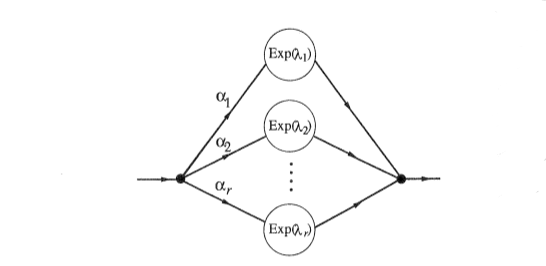
\includegraphics[scale=0.5]{/home/claudio/eclipse/grafici-stat2/alari/mixtureDistribution}
\par\end{center}

$Y$ has an $r-$stage hyperexponential distribution!

\end{frame}

\begin{frame}{Conditional Distribution and Expectation}{Mixture
distributions}

In general the conditional distribution of $Y$ does not have to be
exponential! Denoting $f_{Y\mid X}(y\mid i)=f_{Y_{i}}(y)$ and $F_{Y\mid X}(y\mid i)=F_{i}(y)$
then the unconditional pdf of $Y$ is 
\[
f_{Y}(y)=\sum_{i=1}^{r}\alpha_{i}f_{i}(y)
\]
 and the unconditional CDF of $Y$ is
\[
F_{Y}(y)=\sum_{i=1}^{r}\alpha_{i}F_{i}(y).
\]
Applying the definition of the mean and higher moments we obtain

\begin{eqnarray*}
E[Y] & = & \sum_{i=1}^{r}\alpha_{i}E[Y_{i}],\\
E[Y^{k}] & = & \sum_{i=1}^{r}\alpha_{i}E[Y_{i}^{k}].
\end{eqnarray*}


\end{frame}

\begin{frame}{Conditional Distribution and Expectation}
\begin{itemize}
\item If $X$ and $Y$ are continuous random variables, we can for instance
compute the conditional density $f_{Y\mid X}$. 
\item Since $f_{Y\mid X}$ has all properties of a density function of a
continuous random variable, we can talk about its moments.
\item Its mean (if exists) is called the conditional expectation of $Y$
given $X=x$ and is denoted $E[Y\mid X=x]$ or $E[Y\mid x]$:
\begin{eqnarray*}
E[Y\mid x] & = & \begin{cases}
\int_{-\infty}^{\infty}yf(y\mid x)dy, & \mbox{ if }0<f(x)<\infty\\
0 & \mbox{otherwise.}
\end{cases}
\end{eqnarray*}

\item In case the random variables $X$ and $Y$ are discrete, $E[Y\mid x]$
is defined as
\[
E[Y\mid X=x]=\sum_{y}yP(Y=y\mid X=x)=\sum_{y}yp_{Y\mid X}(y\mid x).
\]

\end{itemize}
\end{frame}

\begin{frame}{Conditional Distribution and Expectation}

Similar arguments hold when $X$ and $Y$ are discrete. The conditional
expectation is then defined as
\[
E[Y\mid X=x]=\sum_{y}yP(Y=y\mid X=x)=\sum_{y}yp_{Y\mid X}(y\mid x).
\]

\begin{definition}%{}
The quantity 
\[
m(x)=E[Y\mid x]
\]
considered as a function of $x$ is known as the \emph{regression
function} of $Y$ on $X$.
\end{definition}%{}
\end{frame}

\begin{frame}{Conditional Distribution and Expectation}
\begin{definition}%{}
The conditional expectation of a function $\phi(Y)$ is defined as
\[
E[\phi(Y)\mid X=x]=\begin{cases}
\int_{-\infty}^{\infty}\phi(y)f_{Y\mid X}(y\mid x)dy, & \mbox{if }Y\mbox{ is continuous,}\\
\sum_{i}\phi(y_{i})p_{Y\mid X}(y_{i}\mid x), & \mbox{if }Y\mbox{ is discrete.}
\end{cases}
\]


We may take expectation of the regression function to obtain the unconditional
expectation of $\phi(Y)$

\[
E[\phi(Y)]=\begin{cases}
\sum_{x}E[\phi(Y)\mid X=x]p_{X}(x), & \mbox{if }X\mbox{ is discrete,}\\
\int_{-\infty}^{\infty}E[\phi(Y)\mid X=x]f_{X}(x)dx, & \mbox{\mbox{if }\ensuremath{X}\mbox{ is continuous}.}
\end{cases}
\]
This last formula is known as the \textbf{theorem of total expectation}.
\end{definition}%{}
\end{frame}

\section{Limit Theorems}

\subsection{Definitions}

\begin{frame}{Limit Theorems}
\begin{theorem}%{}
(Chebyshev) Let $X$ be a random variable with expected value $\mu$
and finite variance $\sigma^{2}<\infty$. The, for all $t>0$, the
following inequality holds

\[
P\left(\mid X-\mu\mid\geq t\right)\leq\frac{\sigma^{2}}{t^{2}}.
\]
\end{theorem}%{}
\begin{definition}%{}
(Convergence in probability) Let $\left\{ X_{n}\right\} _{n\in\mathbb{N}}$
be a sequence of random variables. We say that the sequence converges
in probability to $c\in\mathbb{R}$, write $X_{n}\underset{p}{\rightarrow}c$
or $p\lim X_{n}=c$, if, for all $\epsilon>0$ 

\[
\lim_{n\rightarrow\infty}P\left(\mid X_{n}-c\mid\geq\epsilon\right)=0.
\]

\end{definition}%{}
\end{frame}

\begin{frame}{Limit Theorems}
\begin{theorem}%{}
Let $\left\{ X_{n}\right\} _{n\in\mathbb{N}}$ be a sequence of random
variables with common expectation $\mu$ and finite variance $\sigma_{n}^{2}<\infty$.
If $\lim_{n\rightarrow\infty}\sigma_{n}^{2}=0$, then 

\[
X_{n}\underset{p}{\rightarrow}\mu.
\]
\end{theorem}%{}
\begin{proof}%{}
Apply Chebyshev inequality.\end{proof}%{}
\begin{example}%{}
Let $\left\{ X_{n}\right\} _{n\in\mathbb{N}}$ be an $i.i.d.\sim(\mu,\sigma^{2})$
(independent and identically distributed) sequence of random variables.
Define the sequence $\overline{X}_{n}=\frac{1}{n}\sum_{i=1}^{n}X_{i}$.
From the linearity of the expectation and the properties of the variance
we know that $\bar{X}_{n}\sim(\mu,\frac{\sigma^{2}}{n})$. The sequence
$\left\{ \bar{X}_{n}\right\} _{n\in\mathbb{N}}$ converges in probability
to $\mu$: $p\lim\bar{X}_{n}=\mu$. 
\end{example}%{}
\end{frame} 

\begin{frame}{Limit Theorems}

The result in the previous Example is also known as the \textbf{weak
law of large numbers} (WLLN). In order for the WLLN to apply the existence
of the second moment (the variance) is not required. The WLLN holds
just under the assumption that the $\left\{ X_{n}\right\} _{n\in\mathbb{N}}$
$i.i.d.$ sequence have finite expected value $\mu$.
\begin{theorem}%{}
Consider two sequences $\left\{ X_{n}\right\} _{n\in\mathbb{N}}$
and $\left\{ Y_{n}\right\} _{n\in\mathbb{N}}$ of random variables
converging in probability to $a<\infty$ and $b<\infty$, respectively.
Then\end{theorem}%{}
\begin{enumerate}
\item $p\lim\left(X_{n}+Y_{n}\right)=p\lim X_{n}+p\lim Y_{n}=a+b$.
\item $p\lim\left(X_{n}\cdot Y_{n}\right)=p\lim X_{n}\cdot p\lim Y_{n}=a\cdot b$.
\item $b\ne0$, 
\[
p\lim\left(\frac{X_{n}}{Y_{n}}\right)=\frac{p\lim X_{n}}{p\lim Y_{n}}=\frac{a}{b}.
\]

\item Function $g$ continuous in $a:$ $p\lim g(X_{n})=g\left(p\lim X_{n}\right)=g(a).$
\end{enumerate}
\end{frame} 

\subsection{Standardization}

\begin{frame}{Limit Theorems}
\begin{definition}%{}
(Standardization) Let $X$ be a random variable with expected value
$\mu$ and finite variance $\sigma^{2}$. The location and scale trasform
\[
Z=\frac{X-\mu}{\sigma}
\]
defines the standardization of $X$. From the properties of expectation
it is straightforward to prove that $Z\sim(0,1)$.\end{definition}%{}
\begin{example}%{}
Let $\left\{ X_{n}\right\} _{n\in\mathbb{N}}$ be an indipendent sequence
of random variables with $X_{n}\sim(\mu,\sigma^{2})$ for all $n\in\mathbb{N}$.
Define the sequence $\overline{X}_{n}=\frac{1}{n}\sum_{i=1}^{n}X_{i}$.
Then 
\[
Z_{n}=\frac{\sqrt{n}\left(\overline{X}_{n}-\mu\right)}{\sigma}\sim(0,1)\mbox{ for all }n\in\mathbb{N}.
\]

\end{example}%{}
\end{frame} 

\subsection{Central Limit Theorem}

\begin{frame}{Limit Theorems}
\begin{theorem}%{}
The Central Limit Theorem (CLT). Let $\left\{ X_{n}\right\} _{n\in\mathbb{N}}$
be independent random variables with a finite mean $E[X_{n}]=\mu_{n}$
and a finite variance $Var(X_{n})=\sigma_{n}^{2}$. Define the normalized
random variable

\[
Z_{n}=\frac{\sum_{i=1}^{n}X_{i}-\sum_{i=1}^{n}\mu_{i}}{\sqrt{\sum_{i=1}^{n}\sigma_{i}^{2}}}
\]
 so that $E[Z_{n}]=0$ and $Var(Z_{n})=1$ for all $n$. Then under
regularity conditions the limiting distribution of $Z_{n}$ is standard
normal, denoted $Z_{n}\rightarrow N(0,1),$ i.e.

\[
\lim_{n\rightarrow\infty}F_{Z_{n}}(t)=\lim_{n\rightarrow\infty}P(Z_{n}\leq t)=\int_{-\infty}^{t}\frac{1}{\sqrt{2\pi}}e^{-y^{2}/2}dy.
\]
Remark: the special condition $X_{n}$ independent with $Var(X_{n})=\sigma^{2}$
for all $n$ is sufficient for the CTL to apply.
\end{theorem}%{}
\end{frame} 

\begin{frame}{Limit Theorems}

exercises ...

\end{frame} 

\section{Statistical inference}

\subsection{Parameter Estimation}

\begin{frame}{Parameter estimation}

The object under study is 
\begin{enumerate}
\item the probability distribution function $F$ of a random experiment
or random variable $X$, or
\item the statistical distribution function $F$ of a given attribute of
a population of individuals, users, devices, ... .
\end{enumerate}
We assume that $F$ is known up to a vector of unknown parameters
$\theta$.
\begin{definition}%{}
The family of distributions $\mathcal{P}=\{F_{\theta}\}_{\Theta\subseteq\mathbb{R}^{n}}$,
$n\in\mathbb{N}$ finite, is called parametric model. The parametric
model is usually specified in terms of probability mass or density
functions.
\end{definition}%{}
\end{frame}

\begin{frame}{Parameter estimation}
\begin{example}%{}
We assume that the number of e-mails per minute arriving to an e-mail
server follows a Poisson distribution. The Poisson family of distributions
is parametrized by a single parameter $\lambda>0$
\[
\mathcal{P}=\left\{ p_{\lambda}(j)=\frac{\lambda^{j}}{j!}\exp^{-\lambda},\; j=0,1,\ldots\mid\lambda>0\right\} .
\]

\end{example}%{}
\smallskip{}

\begin{example}%{}
The delivery time of the Google search engine is normal distributed.
The Normal family is parametrized by two parameters $\theta=(\mu,\sigma)$
\[
\mathcal{P}=\left\{ f_{\theta}(x)=\frac{1}{\sqrt{2\pi}\sigma}\exp^{-\frac{1}{2\sigma\text{\texttwosuperior}}(x-\mu)^{2}}\;\mid\mu\in\mathbb{R},\:\sigma>0\right\} .
\]

\end{example}%{}
\end{frame}

\begin{frame}{Parameter estimation}
\begin{example}%{}
In the previous Example, instead of assuming the Normal distribution,
we use the Logistic distribution, that is defined by the following
distribution function (in this case $\theta=(\mu,\beta)):$
\[
\mathcal{P}=\left\{ F_{\theta}(x)=\frac{1}{1+\exp^{-(x-\mu)/\beta}}\;\mid\mu\in\mathbb{R},\:\beta>0\right\} .
\]

\end{example}%{}
\smallskip{}

\begin{example}%{}
We are interested in the percentage of female students at USI. The
distribution of the gender attribute of the USI population is Bernoulli
distributed with parameter $\theta\in[0,1]$.
\end{example}%{}
In all previous examples the {}``true'' vector $\theta$ of parameters
identifying the correct distribution within the corresponding family
is \emph{unknown} and must be estimated by means of a sample (a random
drawn subset of the population). 

\end{frame}

\begin{frame}{Parameter estimation}

Parametric estimation theory deals with the problem of approximating
the unknown parameters by means of the information collected from
the sample.
\begin{example}%{}
In order to estimate the percentage of female students we randomly
select $n$ students (sampling with replacement). In this way we obtain
$n$ independent realizations of Bernoulli distributed random variables
$X_{i}$ where 
\[
P(X_{i}="female")=\theta.
\]
Identifying with 1 the female gender, the sample space is composed
by $2^{n}$ points $x=(x_{1},...,x_{n})$, where $x_{i}\in\{0,1\}$
and $p_{\theta}(x)=\theta^{m(x)}(1-\theta)^{n-m(x)}$ with $m(x)=\sum_{i=1}^{n}x_{i}$.
Given a sample $x$ it seems reasonable to estimate $\theta$ by the
proportion of successes i.e. $m(x)/n$.
\end{example}%{}
\end{frame}

\begin{frame}
\begin{definition}%{}
The set of random variables $X_{1},...,X_{n}$ is said to constitute
a \emph{random sample} of size $n$ from the population with the distribution
function $F(x)$, provided that they are $i.i.d.$, i.e. 
\begin{itemize}
\item mutually independent
\item identically distributed
\end{itemize}
with distribution function $F_{X_{i}}(x)=F(x)$ for all $i$ and all
$x$. 
\end{definition}%{}
\end{frame}

\subsection{Estimator}

\begin{frame}{Point estimation problem}

The basic situation in point estimation is as follows.
\begin{itemize}
\item We observe a realization of random variables $X_{1},...,X_{n}$.
\item The joint distribution function of $X_{1},...,X_{n}$ depends on an
unknown parameter $\theta$ that is known to be in some given set
$\Theta$.
\item The problem to find the value of $\theta$ is a problem of point estimation.
\item We estimate $\theta$ by some function of the observations $x_{1},...,x_{n}$.\end{itemize}
\begin{definition}%{}
Any function of the random variables that are being observed, say
$\hat{\Theta}(X_{1},...,X_{n}),$ is called a \emph{statistic}. It
is also called an \emph{estimator of} $\theta$. Since $X_{1},...,X_{n}$
are random variables, $\hat{\Theta}$ is a random variable too. A
particular realization of the estimator, say $\hat{\Theta}(x_{1},...,x_{n}),$
is called an \emph{estimate of }$\theta$ and denoted by $\hat{\theta}$.
\end{definition}%{}
\end{frame}

\begin{frame}{Point estimation problem}

\begin{osservazione}
\begin{itemize}
\item The function $\hat{\Theta}$ must be known, that is, it does not have
to depend on unknown parameters: $\hat{\Theta}=\overline{X}_{n}$
is a statistics, $\hat{\Theta}=\overline{X}_{n}-\mu$ is not a statistics
if $\mu$ is unknown.
\item The distribution of the estimator $\hat{\Theta}$ is called the sampling
distribution.
\item Since the joint distribution of $X_{1},...,X_{n}$ depends on $\theta$,
the sampling distribution will depends on $\theta$ too. 
\end{itemize}
\end{osservazione}
\begin{example}%{}
Let $X_{1},...,X_{n}$ be an $i.i.d.$ sequence of $N(\mu,1)$ distributed
random variables. From the properties of the Normal distribution we
know that the sample distribution of $\hat{\Theta}=\overline{X}_{n}$
is $N(\mu,\frac{1}{n})$.
\end{example}%{}
In many cases the sampling distribution is an unknown function of
$\theta$.

\end{frame} 

\subsection{Unbiased estimator}

\begin{frame}{Point estimation problem}

We would like our estimator of $\theta$ to be exactly $\theta$ on
average. 
\begin{definition}%{}
We say that $\hat{\Theta}(X_{1},...,X_{n})$ is an unbiased estimator
of $\theta$ if 
\[
E\left[\hat{\Theta}(X_{1},...,X_{n})\right]=\theta.
\]
\end{definition}%{}
\begin{example}%{}
The function
\[
\hat{\Theta}(X_{1},...,X_{n})=\frac{1}{n}\sum_{i=1}^{n}(X_{i}-\bar{X})^{2}
\]
is an estimator of the population variance. It is possible to show
(see Trivedi, page 642) that this estimator is biased, i.e.
\[
E\left[\hat{\Theta}(X_{1},...,X_{n})\right]=\sigma^{2}-\frac{1}{n}\sigma^{2}\neq\sigma^{2}.
\]

\end{example}%{}
\end{frame} 

\begin{frame}{Point estimation problem}
\begin{example}%{}
The formula 
\[
\hat{\Theta}(X_{1},...,X_{n})=\sum_{i=1}^{n}a_{i}X_{i}
\]
 is an unbiased estimator of the expected value $\mu=E[X]$ provided
that the real weights $a_{i}$ satisfy the condition $\sum_{i=1}^{n}a_{i}=1$.\end{example}%{}
\begin{itemize}
\item The previous example shows that many unbiased estimators of the same
parameter may exist.
\item We need a criterion to choose the {}``best'' unbiased estimator.
\item Recall that if $\hat{\Theta}$ is unbiased, then from chebyshev's
inequality
\[
P\left(|\hat{\Theta}-\theta|\geq\epsilon\right)\leq\frac{Var[\hat{\Theta}]}{\epsilon^{2}}\mbox{ for }\epsilon>0.
\]

\end{itemize}
\end{frame}

\subsection{Efficiency}

\begin{frame}{Point estimation problem}
\begin{definition}%{}
\textbf{Efficiency}. An estimator $\hat{\Theta}_{1}$ is said to be
a more efficient estimator of the parameter $\theta$ than the estimator
$\hat{\Theta}_{2}$, provided that
\begin{enumerate}
\item $\hat{\Theta}_{1}$ and $\hat{\Theta}_{2}$ are both unbiased estimators
of $\theta$;
\item $Var[\hat{\Theta}_{1}]\leq Var[\hat{\Theta}_{2}]$, for all $\theta\in\Theta$;
\item $Var[\hat{\Theta}_{1}]<Var[\hat{\Theta}_{2}]$, for some $\theta\in\Theta$.
\end{enumerate}
\end{definition}%{}
\begin{example}%{}
The sample mean 
\[
\bar{X}=\frac{1}{n}\sum_{i=1}^{n}X_{i}
\]
is the most efficient (minimum-variance) linear estimator of the population
mean $\mu$ (provided $\mu$ exists). We also say that $\bar{X}$
is BLUE\emph{ (Best Linear Unbiased Estimator) for $\mu$} (see Trivedi,
page 644).
\end{example}%{}
\end{frame}

\subsection{Consistency}

\begin{frame}{Point estimation problem}

As in the case of the sample mean, the variance of the sampling distribution
of an estimator generally decreases with increasing $n$. This fact
leads us to the following property of an estimator.
\begin{definition}%{}
\textbf{Consistency}. An estimator $\hat{\Theta}$ of the parameter
$\theta$ is said to be consistent if $p\lim\hat{\Theta}=\theta$,
i.e. if
\[
\lim_{n\to\infty}P(|\hat{\Theta}-\theta|\geq\epsilon)=0.
\]

\end{definition}%{}
From the Chebyshev inequality we conclude that any unbiased estimator
$\hat{\Theta}$ of the parameter $\theta$ such that 
\[
\lim_{n\to\infty}Var[\hat{\Theta}]=0
\]
 is consistent.

\end{frame}

\begin{frame}{Point estimation problem}
\begin{example}%{}
The empirical distribution function, 
\[
\hat{F}(x)=\frac{\#\mbox{ observations }\leq x}{n}
\]

\end{example}%{}
is for all $x\in\mathbb{R}$ a consistent estimator of the true distribution
function $F(x)$. Proof: see Trivedi, page 645. 

\end{frame} 

\subsection{Method of least squares}

\begin{frame}{Method of least squares}

Starting point:
\begin{itemize}
\item We observe a random sample $y_{1}$, ..., $y_{n}$ from a population
with distribution function $F$.
\item We are interested in estimating the mean $\theta$ of the distribution.
\end{itemize}
We rewrite our model as 
\[
y_{i}=\theta+\epsilon_{i}
\]
where $\epsilon_{i}:=y_{i}-\theta$ is the zero mean deviation error
of the $i-th$ observation from the mean of the underlying distribution.
Note that $Var[\epsilon_{i}]=Var[y_{i}]=\sigma\text{\texttwosuperior}$
for all observations. One possible criterion to estimate $\theta$
is to choose an estimate such that the sum of squared errors is as
small as possible, i.e.
\[
\hat{\theta}(y_{1},...,y_{n})=\min_{\theta}\sum_{i=1}^{n}\epsilon_{i}^{2}=\min_{\theta}\sum_{i=1}^{n}(y_{i}-\theta)^{2}.
\]


The solution is $\hat{\theta}(y_{1},...,y_{n})=\bar{y}$ the mean
of the sample!

\end{frame}

\begin{frame}{Method of least squares}

We can extend the argument to the case where the expected value of
the random variable $Y_{i}$ depends on a concomitant \textbf{deterministic}
and \textbf{observable} variable $x_{i}$. If the dependence is linear,
we have that 
\[
E[Y_{i}]=\theta_{1}+\theta_{2}x_{i},
\]
where $\theta'=(\theta_{1},\theta_{2})$ is a vector of unknown parameters.
As before, under this further assumptions we can write our model as
\[
y_{i}=\theta_{1}+\theta_{2}x_{i}+\epsilon_{i}
\]
and estimate $\theta_{1}$ and $\theta_{2}$ by those number minimizing
\[
\min_{\theta}\sum_{i=1}^{n}\epsilon_{i}^{2}=\min_{\theta}\sum_{i=1}^{n}(y_{i}-\theta_{1}-\theta_{2}x_{i})^{2}.
\]


\end{frame} 

\begin{frame}{Method of least squares}

Finally, we can generalize the argument to the case of $K$ explanatory
variables $x_{i}'=(x_{i,1},\ldots,x_{i,K})$. This means that, for
the $i-th$ observation $y_{i}$, the model is 
\begin{eqnarray*}
y_{i} & = & \theta_{1}x_{i,1}+\theta_{2}x_{i,2}+...+\theta_{K}x_{i,K}+\epsilon_{i}\\
y_{i} & = & x_{i}'\theta+\epsilon_{i}
\end{eqnarray*}
We can rewrite the model in a more compact way using matrix notation
\[
\underset{(n\times1)}{y}=\underset{(n\times K)}{X}\underset{(K\times1)}{\theta}+\underset{(n\times1)}{\epsilon}
\]
where $y'=(y_{1},...,y_{n})$, $\epsilon'=(\epsilon_{1},...,\epsilon_{n})$
and 
\[
X=\left[\begin{array}{c}
x_{1}'\\
x_{2}'\\
\vdots\\
x_{n}'
\end{array}\right]=\left[\begin{array}{cccc}
x_{1,1} & x_{1,2} & \ldots & x_{1,K}\\
x_{2,1} & x_{2,2} & \ldots & x_{2,K}\\
\vdots & \vdots & \ddots & \vdots\\
x_{n,1} & x_{n,2} & \ldots & x_{n,K}
\end{array}\right].
\]


\end{frame} 

\begin{frame}{Method of least squares}

Again, the estimates of the $K$ parameters $\theta_{j}$, $j=1,...,K$
are obtained by minimizing the sum of squared
\[
\min_{\theta}\sum_{i=1}^{n}\epsilon_{i}^{2}=\min_{\theta}\epsilon'\epsilon=\min_{\theta}\left(y-X\theta\right)'\left(y-X\theta\right).
\]

\begin{itemize}
\item This method of estimation is called the \emph{method of least squares}.
\item Any minimizing value $\hat{\theta}(y)$ is called the \emph{least-square
estimate} of $\theta$.
\item The function $\hat{\theta}:\mathbb{R}^{n}\rightarrow\mathbb{R}^{K}$
is a \emph{least-squares estimator}.
\end{itemize}
The solution of the minimization problem is obtained by differentiating
with respect to $\theta$ the quadratic form $\left(y-X\theta\right)'\left(y-X\theta\right)$
and solving the first order conditions 
\[
X'X\theta=X'y.
\]


\end{frame} 

\begin{frame}{Method of least squares}

Any solution of the system of equations $X'X\theta=X'y$ is a least-square
estimate. If rank $X=K$, then $X'X$ is non-singular and the unique
least-square estimate is 
\[
\hat{\theta}(y)=(X'X)^{-1}X'y.
\]


If rank $X<K$, then $X'X$ is singular and there is a family of least-square
estimates.

\begin{esercizio}

Assume the following regression model
\[
y_{i}=\theta+\epsilon_{i}\quad i=1,\ldots,n.
\]

\begin{enumerate}
\item Express the model in matrix form and give the dimension and the content
of the matrix $X$.
\item Show that $\hat{\theta}(y)=(X'X)^{-1}X'y=\bar{y}.$
\end{enumerate}
\end{esercizio}

\end{frame} 

\begin{frame}{Method of least squares}

\begin{esercizio}

Assume the following regression model
\[
y_{i}=\theta_{1}+\theta_{2}x_{i}+\epsilon_{i}\quad i=1,\ldots,n.
\]

\begin{enumerate}
\item Express the model in matrix form and give the dimension and the content
of the matrix $X$ in terms of the constant $1$ and the explanatory
variable $x_{i}$, $i=1,...,n$.
\item Show that $\hat{\theta}_{1}=\bar{y}-\hat{\theta}_{2}\bar{x}$ and
$\hat{\theta}_{2}=\frac{\sum_{i}(x_{i}-\bar{x})y_{i}}{\sum_{i}(x_{i}-\bar{x})^{2}}$. 
\end{enumerate}
\end{esercizio}

\end{frame} 

\subsection{Maximum likelihood estimation}

\begin{frame}{Maximum likelihood estimation}

Suppose that each night a certain lion has three possible states of
activity:
\begin{enumerate}
\item very active, denoted by $\theta_{1}$;
\item moderately active, denoted by $\theta_{2}$;
\item lethargic, denoted by $\theta_{3}$.
\end{enumerate}
Each night this lion eats $i$ people with probability $p(i|\theta),\:\theta\in\Theta$
where $\Theta=\{\theta_{j},\; j=1,2,3\}$. The numerical values are
given in the following table:

\begin{center}
\begin{tabular}{|c|cccc|}
\hline 
$i$ & 0 & 1 & 2 & 3\tabularnewline
\hline 
$p(i|\theta_{1})$ & 0.00 & 0.05 & 0.05 & 0.90\tabularnewline
$p(i|\theta_{2})$ & 0.05 & 0.05 & 0.80 & 0.10\tabularnewline
$p(i|\theta_{3})$ & 0.90 & 0.08 & 0.02 & 0.00\tabularnewline
\hline 
\end{tabular}
\par\end{center}

\textbf{Question:} If we know that $X=i_{0}$ people were eaten last
night, how should we estimate the lion's activity state?

\end{frame} 

\begin{frame}{Maximum likelihood estimation}

\textbf{Answer:} take as the estimate of $\theta$ that $\theta_{j}\in\Theta$
for which the probability $p(i_{0}|\theta)$ is largest! In this example
we have $\hat{\theta}(i_{0}=0)=\theta_{3}$, $\hat{\theta}(i_{0}=1)=\theta_{3}$,
$\hat{\theta}(i_{0}=2)=\theta_{2}$, $\hat{\theta}(i_{0}=3)=\theta_{1}$.

\smallskip{}
Suppose that we know for sure that $\theta\in\Theta'=\{\theta_{1},\theta_{2}\}$.
The estimate is no longer unique since it can be either $\theta_{1}$
or $\theta_{2}$.
\begin{definition}%{}
Let $X_{1},...,\; X_{n}$be $n$ random variables with distribution
function $F(x_{1},...,x_{n}|\theta)$ where $\theta\in\Theta$ is
unknown. The \emph{likelihood function} is 

\[
L(\theta)=\left\{ \begin{array}{cc}
f_{X_{1},...,X_{n}}(x_{1},...,x_{n}|\theta), & \mbox{if \ensuremath{F} has a density function \ensuremath{f},}\\
p_{X_{1},...,X_{n}}(x_{1},...,x_{n}|\theta), & \mbox{if \ensuremath{F} has a prob. function \ensuremath{p}. }
\end{array}\right.
\]
Any $\hat{\theta}=\hat{\Theta}(X_{1},...,X_{n})\in\Theta$ such that
\[
L(\hat{\theta})=sup\{L(\theta):\theta\in\Theta\}
\]
is called \emph{maximum-likelihood estimator} (MLE) of $\theta$.
\end{definition}%{}
\end{frame}

\begin{frame}{Maximum likelihood estimation}

\textbf{Remark:} Those $\hat{\theta}$'s that maximize the likelihood
function $L(\theta)$ are precisely those that maximize the \emph{log-likelihood
function} $\log L(\theta).$ It turns out that maximization of the
log-likelihood function is often easier.

\begin{center}
\includegraphics[width=12.5cm]{\string"example1 maximumLikelihood\string".eps}
\par\end{center}

\end{frame}

\begin{frame}{Maximum likelihood estimation}

\begin{center}
\includegraphics[width=12.4cm]{\string"example2 maximumLikelihood\string".eps}
\par\end{center}

\begin{center}
\includegraphics[width=12.4cm]{\string"example3 maximumLikelihood\string".eps}
\par\end{center}

\end{frame} 

\begin{frame}{Maximum likelihood estimation}

\begin{center}
\includegraphics[width=12.5cm]{\string"example4 maximumLikelihood\string".eps}
\par\end{center}

\begin{center}
\includegraphics[width=12.5cm]{\string"example5 maximumLikelihood\string".eps}
\par\end{center}

\end{frame} 

\begin{frame}{Maximum likelihood estimation}

\begin{center}
\includegraphics[width=12.3cm]{\string"example6 maximumLikelihood\string".eps}
\par\end{center}

\end{frame} 

\begin{frame}{Maximum likelihood estimation}

\begin{center}
\includegraphics[width=12.3cm]{\string"example7 maximumLikelihood\string".eps}
\par\end{center}

\begin{center}
\includegraphics[width=12.3cm]{\string"example8 maximumLikelihood\string".eps}
\par\end{center}

\end{frame} 

\subsection{The method of moments}

\begin{frame}{The method of moments}

\begin{center}
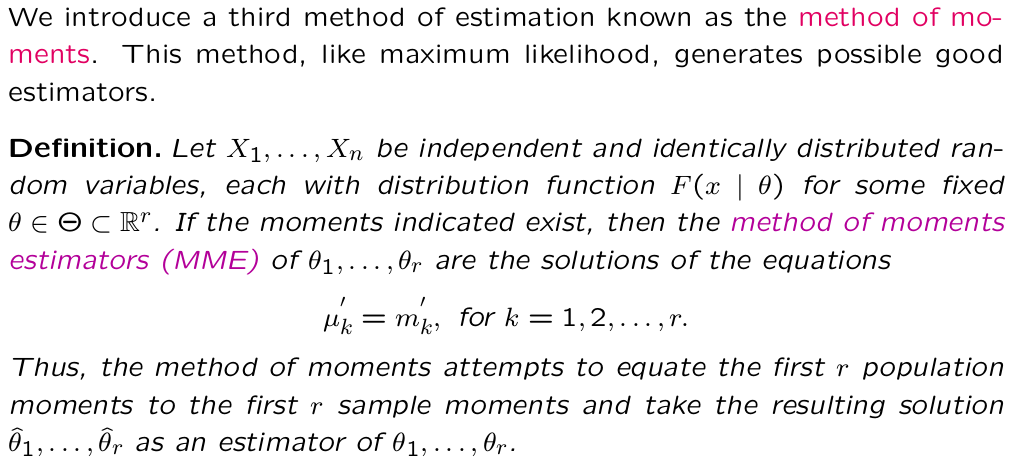
\includegraphics[width=12.5cm]{mme1}
\par\end{center}

\end{frame} 

\begin{frame}{The method of moments}

\begin{center}
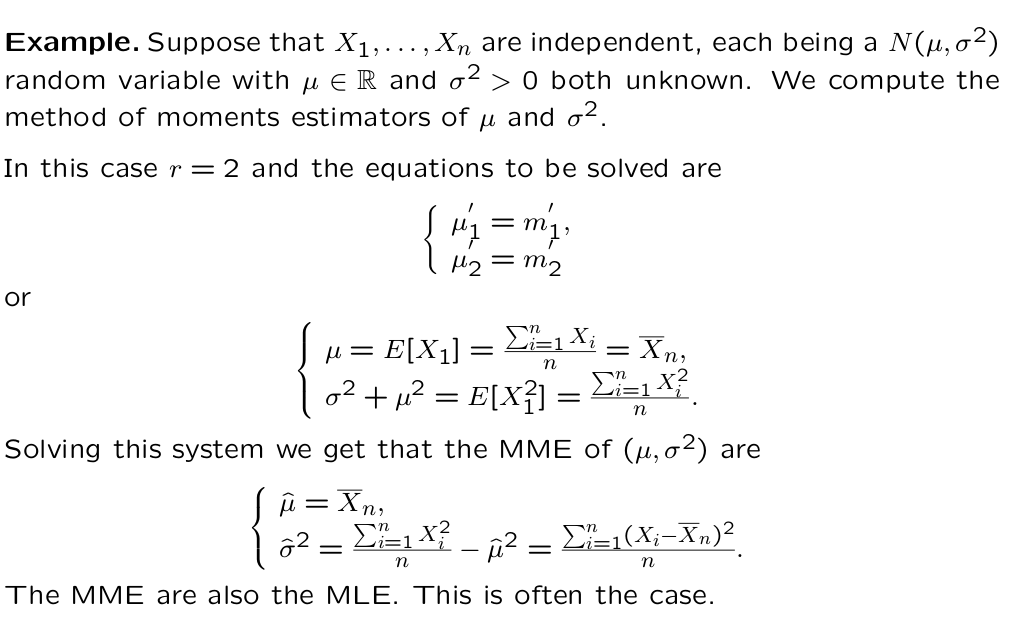
\includegraphics[width=12.3cm]{mme2}
\par\end{center}

\end{frame} 

\begin{frame}{The method of moments}

\begin{center}
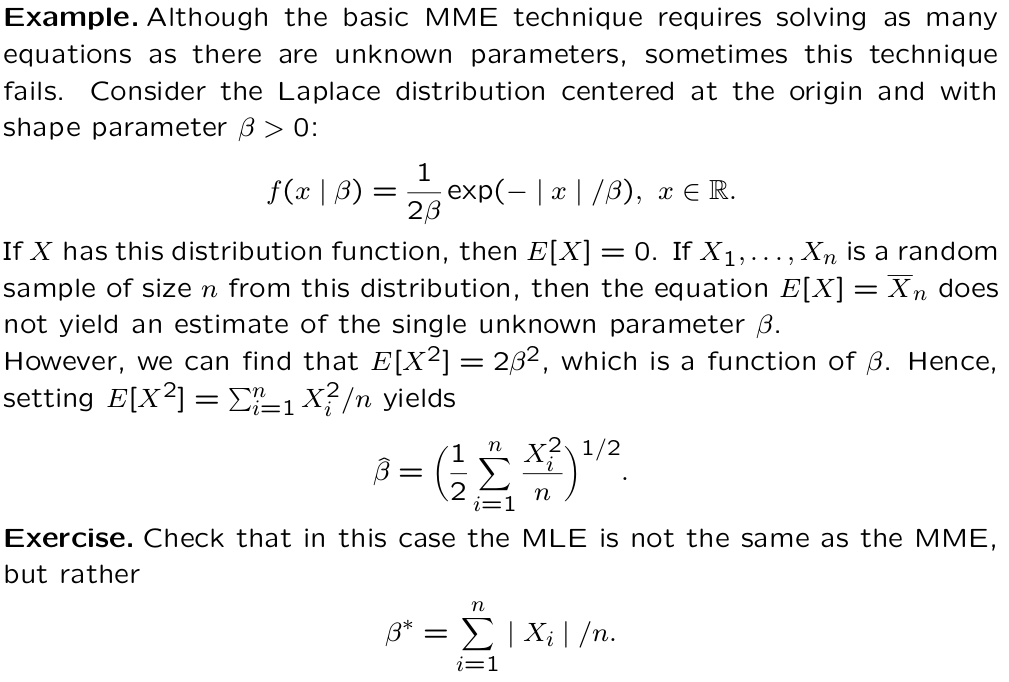
\includegraphics[height=8cm]{mme3}
\par\end{center}

\end{frame} 
\end{document}
